\section*{4. Memorization vs.\ Generalization (EC7)}

\subsection*{Problem \& Approach}
Main HW3 trains on $\sim$1,300 emoji for 500 epochs and generates new samples via Euler sampling---but does the model \emph{generalize} or \emph{memorize}? EC7 tests this for the same architecture and training recipe (x-pred, no time conditioning), using four experiments grounded in Carlini et al.\ (2023) and Somepalli et al.\ (2023). Pixel-space L2 nearest-neighbor distance is our replication metric at 32$\times$32.

We train for 400 epochs (vs.\ main HW3's 500) and compare generated samples against the same training set main HW3 uses.

\subsection*{Results}

\begin{table}[h]
\centering
\begin{tabular}{l l c l}
\toprule
\textbf{Experiment} & \textbf{Metric} & \textbf{Result} & \textbf{Implication for Main HW3} \\
\midrule
NN replication & median gen$\to$train & 19.83 & no copy spike \\
               & median train$\to$train & 21.64 & natural spacing \\
\midrule
Held-out test  & gen$\to$seen & 23.11 & not memorizing seen half \\
               & gen$\to$held-out & 23.48 & generalizes to unseen \\
\bottomrule
\end{tabular}
\caption{Memorization metrics for a model trained with main HW3's recipe.}
\label{tab:ec7_metrics}
\end{table}

\begin{figure}[h]
    \centering
    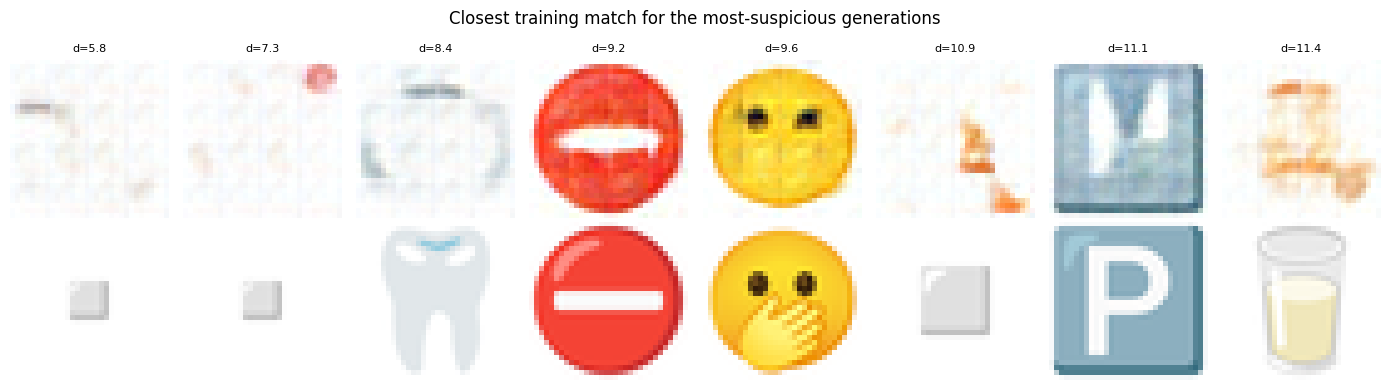
\includegraphics[width=0.95\textwidth]{figures/ec7_nn_pairs.png}
    \caption{Closest training matches for the most suspicious generations---similar to but not identical copies of main HW3 training data.}
    \label{fig:ec7_pairs}
\end{figure}

\begin{figure}[h]
    \centering
    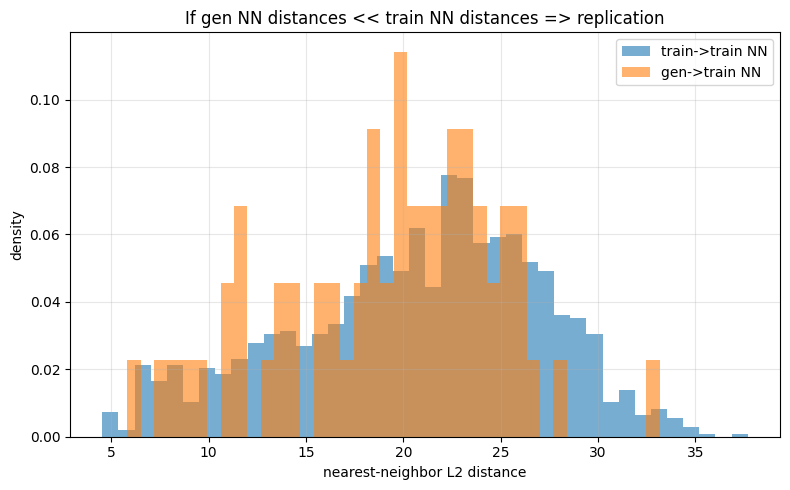
\includegraphics[width=0.48\textwidth]{figures/ec7_nn_hist.png}
    \hfill
    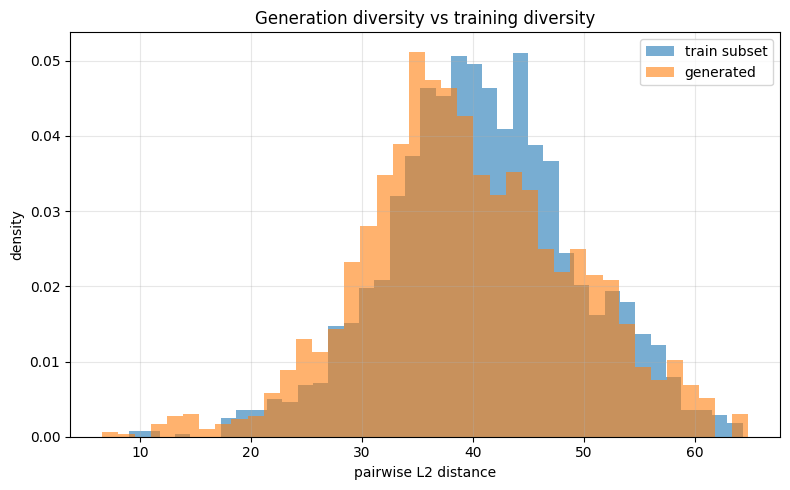
\includegraphics[width=0.48\textwidth]{figures/ec7_diversity.png}
    \caption{Left: NN histogram (gen vs.\ train baseline). Right: diversity matches training set.}
    \label{fig:ec7_hist_div}
\end{figure}

\begin{figure}[h]
    \centering
    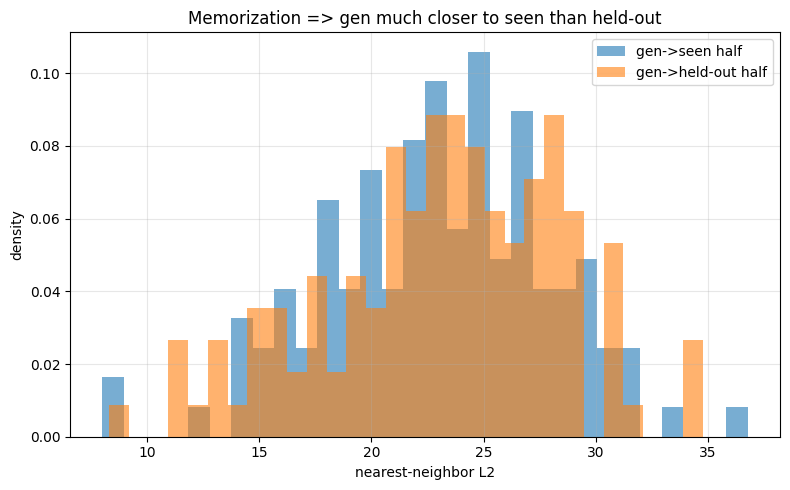
\includegraphics[width=0.48\textwidth]{figures/ec7_heldout.png}
    \hfill
    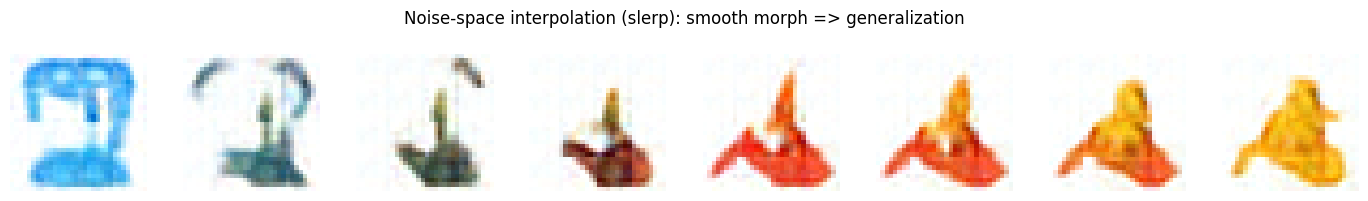
\includegraphics[width=0.48\textwidth]{figures/ec7_interpolation.png}
    \caption{Left: held-out test. Right: smooth noise interpolation (learned manifold, not lookup).}
    \label{fig:ec7_held_interp}
\end{figure}

\subsection*{Discussion}
\textbf{Verdict for main HW3's training setup: generalization, not memorization.}

\begin{itemize}
    \item Gen$\to$train NN distances (19.83) match the train$\to$train baseline (21.64)---main HW3's generations are not near-exact copies.
    \item Held-out distances are comparable (23.11 vs.\ 23.48), so the model does not preferentially reproduce seen emoji.
    \item Smooth noise-space interpolation indicates a learned continuous manifold, consistent with the diverse samples in main HW3's Viz 2b (Figure~\ref{fig:main_samples}).
\end{itemize}

Main HW3's occasional fuzzy or repetitive-looking samples are more likely limited model capacity or sampling error than verbatim memorization. A stronger test would apply the same metrics directly to main HW3's saved 500-epoch checkpoint.
